A ranking is an ordered subset of measures of the same quantity, between which exists an order relation. Rankings allow us to obtain complex informations with the use of very little data, since the information is contained in the order of the values. \\ 
An example of the use of rankings can be found in web pages, where the search engine shows to the user the results of the search, and the results are ordered depending on their relevance, so to allow them to find the desired information as quickly as possible. \\
In this example, the quantity is the relevance of a result to the search. \\ \\
Another example is the population of cities. The graph below shows the population of the 300 bigges cities in Europe. The graph is in log-log scale, and since it shows a straight line, it means that the distribution is a power law distribution. \\
\begin{center}
	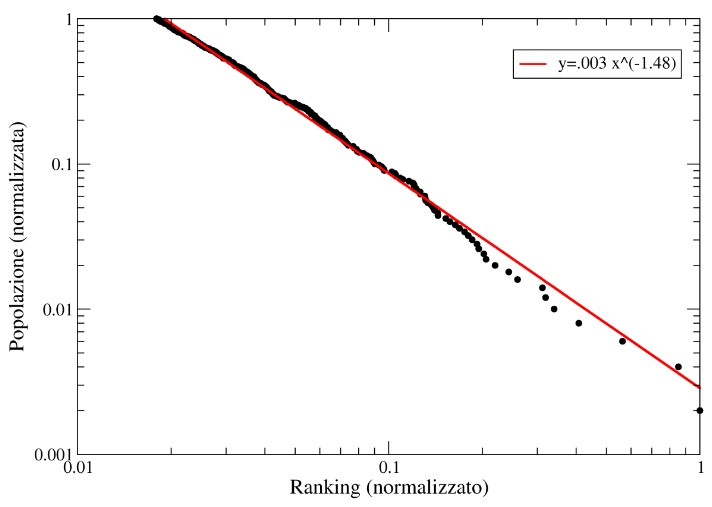
\includegraphics[scale=0.65]{cities_ranking.jpg}
\end{center}
This can be explained considering the fact that, storically, the population used to migrate towards the biggest cities of the country, because there were more job opportunities. Thus one can say that big cities have a preferential attatchment. \\ \\ 
Let $x$ be a random variable and $\{x_1,x_2, . . . , x_N\}$ a sample of experimental observations of the variable, ordered in such a way that $x_1 \geq x_2 \geq . \ . \ . \ \geq x_N$. \\ 
Then, the ranking distribution is created by assigning to the position $j$ in the order the corresponding value in the sampe, which is given by the map $x_j = f(j)$. Also, usually the elements are normalized like $y_j = x_j/x_1$. \\ 
By definition, $j/N$ is the frequency of the event $\{x \ | \ x \geq x_j \}$, that is, the probability that the variable $x$ has a value larger that $x_j$ for larger values of $j$. \\ \\
The cumulative distribution is defined as $F(x) = P\{u \ | \ u \leq x_j\}$, that is, the probability that the value $u$ is smaller that $x$. Of course, this probability is equal to the integral of the distribution in the range $[-\infty,x]$. \\
The relation between the frequency $j/N$ and the cumulative distribution is given by:
$$
	F(x_j) = 1 - \frac{j}{N} = 1 - \frac{J(x_j)}{N}
$$
where $J(x_j)$ is the inverse of the ranking, so it's the function that returns the position of a certain value of $x$ in the sample's order. \\
Since the cumulative distribution is the integral of the probability distribution, the latter can be obtained by differentiating the first:
$$
	p(x) = \frac{dF}{dx} \ \ \longrightarrow \ \ p(x) = -\frac{1}{N} \frac{dJ}{dx}
$$
